%%%%%%%%%%%%%%%%%%%%%%%%%%%%%%%%%%%%%%%%%%%%%%%%%%%%%%%%%%%%%%%%%%%%%%%%%%%%%%%%

\documentclass{article}
\pdfpagewidth=8.5in
\pdfpageheight=11in
% The file ijcai18.sty is the style file for IJCAI-18 (same as ijcai08.sty).
\usepackage{ijcai18}

% Use the postscript times font!
\usepackage{times}
\usepackage{xcolor}
\usepackage{soul}
\usepackage[utf8]{inputenc}
\usepackage[small]{caption}

\usepackage{graphicx}
\usepackage{algorithmic}
\usepackage{algorithm}
\usepackage{paralist}
\usepackage{flushend}
\usepackage{hyperref}
\usepackage{setspace}
\usepackage{enumitem}

\usepackage{amsmath}
\usepackage{amsthm}
\newtheorem{theorem}{Theorem}
\newtheorem*{theorem*}{Theorem}
\newtheorem{proposition}{Proposition}
\newtheorem*{proposition*}{Proposition}
\newtheorem{definition}{Definition}
\newtheorem*{definition*}{Definition}



\title{
  \setstretch{1.15}
  Counterfactual Simulation for Pathway Analysis of
  Rule-Based Models of Signalling Networks
}

\author{
  Jonathan Laurent$^1$,
  Jean Yang$^1$,
  Walter Fontana$^2$, \\
  %
  $^1$ Carnegie Mellon University \\
  $^2$ Harvard Medical School \\
  % 
  \{jonathan.laurent,\ jyang2+\}@cs.cmu.edu, \ 
  % jonathan.laurent@cs.cmu.edu, \ 
  % jyang2+@cs.cmu.edu, \ 
  walter\_fontana@hms.harvard.edu
}
% \setlength\titlebox{2.5in}

%%%%%%%%%%%%%%%%%%%%%%%%%%%%%%%%%%%%%%%%%%%%%%%%%%%%%%%%%%%%%%%%%%%%%%%%%%%%%%%%

%%%%%%%%%%%%%%%%%%%%%%%%%%%%%%%%%%%%%%%%%%%%%%%%%%%%%%%%%%%%
% Formatting macros

%\newcommand{\m}[1]{{\small\textsf{#1}}}
\newcommand{\m}[1]{{\textsc{#1}}}
\newcommand{\TODO}[1]{[\textsl{#1}]}

%%%%%%%%%%%%%%%%%%%%%%%%%%%%%%%%%%%%%%%%%%%%%%%%%%%%%%%%%%%%
% Math Macros

\newcommand{\Nat}{{\mathbb N}}
\newcommand{\Real}{{\mathbb R}}
\newcommand{\eqdef}{\triangleq}

\newcommand{\Prob}[1]{\mathbf{P} \left\{\, #1 \,\right\}}
\newcommand{\ProbParen}[1]{\mathbf{P} \left(\, #1 \,\right)}
\newcommand{\ProbParenSmall}[1]{\mathbf{P}\left(#1\right)}
\newcommand{\CProb}[2]{\Prob{#1 \ |\  #2}}

%%%%%%%%%%%%%%%%%%%%%%%%%%%%%%%%%%%%%%%%%%%%%%%%%%%%%%%%%%%%
% Kappa notations

% Left-hand side and right-hand side of a rule
\newcommand{\RLHS}[1]{L_{#1}}
\newcommand{\RRHS}[1]{R_{#1}}

% State in a trace
%\newcommand{\TSTATE}[2]{\m{State}_{#1}(#2)}
%\newcommand{\TSTATE}[2]{\left[#2\right]^{#1}}
%\newcommand{\TSTATE}[2]{#2^{[#1]}}
%\newcommand{\TSTATE}[2]{#2[#1]}
\newcommand{\TSTATE}[2]{#2\text{\footnotesize$[#1]$}}

% Embeddings and divergent embeddings
\newcommand{\EMBS}[2]{\m{Emb}_{#1}(#2)}
\newcommand{\DEMBS}[2]{\m{Emb}'_{#1}(#2)}
%\newcommand{\EMBS}[2]{\mathcal{E}'_{#1}(#2)}
%\newcommand{\DEMBS}[2]{\mathcal{E}'_{#1}(#2)}

% Executable potential event
\newcommand{\TRIGGERABLE}[2]{#1 \vdash #2}

% Updating a mixture
\newcommand{\UPDATE}[2]{#1\nolinebreak\boldsymbol{\cdot}\nolinebreak#2}
%\newcommand{\UPDATE}[2]{#1 \,!\, #2}

% Time of an event
\newcommand{\TIME}[1]{\textsc{time}(#1)}

%%%%%%%%%%%%%%%%%%%%%%%%%%%%%%%%%%%%%%%%%%%%%%%%%%%%%%%%%%%%
% Macros for counterfactuals

% Altered and counterfactual traces
\newcommand{\ATRAJ}[0]{{T_\iota}}
\newcommand{\CTRAJ}[0]{{T_\iota\,|\,\{T=\tau\}}}

% 'blocked' predicate
\newcommand{\BLOCKED}[2]{\m{blocked}_{#1}[#2]}

% Typical counterfactual statement
\newcommand{\CFST}[0]{\tau \models [\iota] \, \psi}

% Reference trace
%\newcommand{\RefTrace}{trace~(\ref{example-trace})}
%\newcommand{\RefTrace}{trace~\ref{example-trace}}
\newcommand{\RefTrace}{trace~{\small(\ref{example-trace})}}

\begin{document}

\maketitle

% -*- TeX-master: "ijcai18.tex" -*-

\begin{abstract}
  Models based on rules that express local and heterogeneous mechanisms
  of stochastic interactions between structured agents are an
  important tool for investigating the dynamical behavior of complex
  systems, especially in molecular biology. Given a simulated trace of
  events, the challenge is to construct a causal diagram that explains
  how a phenomenon of interest occurred. Counterfactual analysis can
  provide distinctive insights, but its standard definition is not
  applicable in rule-based models because they are not readily
  expressible in terms of structural equations. We provide a semantics
  of counterfactual statements that addresses this challenge by
  sampling counterfactual trajectories that are probabilistically as
  close to the factual trace as a given intervention permits them to
  be. We then show how counterfactual dependencies give rise to
  explanations in terms of relations of enablement and prevention
  between events.
\end{abstract}

\section*{Introduction}\label{sec:intro}

Rule-based modeling languages for molecular biology, such as Kappa
\cite{DanosEtAl-CONCUR07} and BioNetGen \cite{bngl}, or organic
chemistry, such as M{\o}d \cite{moll}, can be used to write
mechanistic models of complex reaction systems. In these approaches,
chemical transformations are represented by local graph-rewrite rules
equipped with stochastic firing rates. In a dynamical simulation,
rules induce a time series of events that might reach a state of
interest in processes like the assembly of a molecular machine, the
activation of a transcription factor, or the synthesis of a specific
chemical compound. While rule-based models provide compactness,
transparency, and the ability of handling combinatorial complexity,
the perhaps most significant advantage lies in their suitability for
causal analysis that takes into account the logically concurrent
nature of interactions.

The causal analysis
\cite{DBLP:conf/fsttcs/DanosFFHH12,DanosEtAl-CONCUR07} of event series
generated by such models provides a formal definition of ``pathway"
and a means for revealing the emergence of pathways from low-level
interactions. These methods take advantage of rule structure to
\begin{inparaenum}[(i)]
\item compress a given simulation trace into a minimal subset of
  events that are necessary and jointly sufficient to replicate a
  phenomenon of interest and
\item highlight the direct causal influences between events, exposing
  the extent of concurrency.
\end{inparaenum}

% There is much more to discuss here.

We propose a distinct but complementary approach based on
\textit{counterfactual reasoning} that improves causal explanations by
\begin{inparaenum}[(i)]
\item being more sensitive to kinetics and
\item properly accounting for the causal impact from inhibition
  between events.
\end{inparaenum}

\section{Motivating example}\label{sec:example}

% Much more to say about Kappa

We illustrate the need for counterfactual reasoning on a toy example
in Kappa. Consider a model with two types of agents, kinases $K$ and
substrates $S$, interacting according to the rules depicted in
Figure~\ref{fig:model}.

% -*- TeX-master: "ijcai18.tex" -*-

\begin{figure}[h]
  \vskip -0.2cm
  \begin{center}
    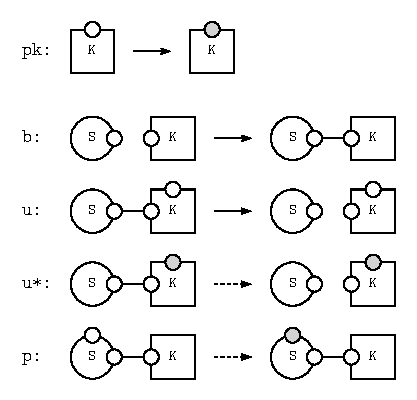
\includegraphics[scale=0.9]{figures/model.pdf}
  \end{center}
  \vskip -0.2cm
  % \caption{A motivating toy model. As usual in Kappa, sites not
  %   mentioned in a rule are left unchanged by it. Instead of naming
  %   sites, we here identify them by their position on an
  %   agent. Phosphorylated sites are shown in gray. Firing rates are
  %   not specified here but dotted arrows indicate \textit{slow}
  %   reactions, whereas solid arrows indicate \textit{fast} reactions.}
  \caption{A motivating toy model. Sites not mentioned in a rule are
    left unchanged by it. \longversion{As in
      Figure~\protect\ref{fig:mixture}, sites are identified by their
      position on an agent.}  Firing rates are not specified, but
    dotted (solid) arrows indicate \textit{slow} (\textit{fast})
    reactions
    $(\lambda_u \gg \lambda_{u^*} \approx \lambda_p)$.}
  \label{fig:model}
\end{figure}


For the sake of simplicity, consider an initial mixture $I$ with only
a single kinase and a single substrate whose sites are free and
unphosphorylated. We then ask: Starting from $I$, \textbf{how} is $p$
triggered ? We are not merely looking for an account of reachability
but rather for causal narratives, that is, collections of necessary
events connected by causal influences.

A stochastic simulation \cite{DanosEtAl-APLAS07} might produce the
following trace (events are labelled by the rules that induced them):
\begin{align}\label{example-trace} b,\ \ u,\ \ pk,\ \ b,\ \ p,\ \
  u^{*},\ \ \cdots
\end{align} Figure~\ref{fig:dumb-story} depicts the causal narrative
explaining the occurrence of $p$ according to existing techniques
\cite{DBLP:conf/fsttcs/DanosFFHH12,DanosEtAl-CONCUR07}. The arrow
between $b$ and $p$ is called an \textit{activation arrow}, meaning
that $b$ modifies an aspect of state (by creating a link) that enables
$p$ to happen.

\begin{figure}[H]
  \vskip -0.8cm
  \begin{center}
    \includegraphics[scale=0.7]{figures/dot/dumb-story.pdf}
  \end{center}
  \vskip -1cm
  \caption{A causal explanation for $p$ in trace
    (\ref{example-trace}).  Events are labelled by the rules that
    induced them. The \emph{init} node corresponds to a special event
    that sets the mixture to its initial state.  }
  \label{fig:dumb-story}
\end{figure}


This narrative, however, is blind to the critical role of $pk$ in the
original trace. Looking at the rules in Figure~\ref{fig:model} one
notes that:
\begin{inparaenum}[(i)]
\item the phosphorylation rule $p$ is slow
\item the average time $K$ and $S$ remain bound depends on whether $K$
  is phosphorylated, as manifest in the two unbinding rules $u$ (fast,
  if $K$ is not phosphorylated) and $u^{*}$ (slow, if $K$ is
  phosphorylated).
\end{inparaenum} It seems reasonable to assert that $p$ would probably
not have happened had $pk$ not happened, as the opportunity for $p$
would have been cut short by a fast unbinding event. We therefore
argue that $pk$, although it does not activate $b$ or $p$ directly,
should be part of a causal narrative for $p$. Reasoning of this kind
is \textit{counterfactual} and can be deployed to define causality
\cite{lewis1974causation,lewis2000causation}.

In section~\ref{sec:counterfactual}, we give a rigorous semantics to
this line of reasoning. In section~\ref{sec:inhibition} we show that
counterfactual statements can be expressed using inhibition arrows,
leading to the explanation shown in Figure~\ref{fig:cex}.

% Therefore, although the causal relevance of $pk$ cannot be justified
by activation arrows, it is supported by a counterfactual statement.
% In the rest of this abstract, we %give a formal semantics to
counterfactual statements and investigate how %they can be used %to
produce more satisfying causal explanations.

\section{Counterfactual simulation}\label{sec:counterfactual}

Counterfactual statements are tricky because their truth is
context-dependent. The statement ``Had it not rained, the driver might
have arrived earlier" can fail to be true in many ways. Intuitively,
how easily the driver could have arrived earlier depends on how great
a departure from actuality is required for it to be case
\cite{Lewis1973}. This is why counterfactual reasoning is tied to
modal logic. The standard approach is to require that the consequent
in a counterfactual be true in some of those possible worlds (in which
the antecedent holds) that \textit{are most similar to the actual
  world}. If the counterfactual statement is true in all of these
worlds, we can replace ``might" with ``would".  We now operationalize
this approach in the context of Kappa traces and interpolate between
``might" and ``would" using probabilities.

We start by formalizing the notion of an intervention. An intervention
$\iota$ (``blocking $pk$" in our example) is a predicate
$\BLOCKED{\iota}{t, e}$ that determines whether or not event $e$ is
blocked at time $t$. Given a predicate $\varphi$ over traces, we write
the proposition \textit{``Had intervention $\iota$ happened in trace
  $\tau$, $\varphi$ would have been true with probability greater than
  $p \in [0,1]$''} as:
\[ \tau \models_p [\iota] \, \varphi.
\]

To give an operational meaning to this statement, we invoke the
continuous time Markov chain (CTMC) semantics of a Kappa model as
defined and implemented in
\cite{DanosEtAl-APLAS07,BoutillierEK17}. For the present purpose it is
conceptually useful to think of a CTMC abstractly in terms of the
random realization of ``potential events". A potential event is a pair
$(r, \xi)$ where $r$ is a rule and $\xi$ an injective mapping from
local agents involved in $r$ to global agents in a huge virtual
mixture of many instances of all possible molecular
species.\footnote{For the sake of simplicity, we assume that no agent
  is created or deleted by a rule.} For every such potential event, we
imagine a bell that rings at a time $t$ drawn from an exponential
distribution $\lambda_r\exp(-\lambda_r t)$, where $\lambda_r$ is the
stochastic rate constant of $r$. A simulation trace can be viewed as
the realization of a random variable $T$ determined by the set
$\omega$ of ring times: Starting with an initial mixture, when a bell
rings at $t$, its associated potential event $(r, \xi)$ transforms the
mixture according to $r$ if $\xi$ yields a valid embedding of the left
hand side of $r$ in the current mixture and time advances by
$t$. Otherwise, time advances and nothing happens---a null
event. Repeat on the resulting mixture.

We can extend this viewpoint to include interventions. For an
intervention $\iota$, we define the random variable $\ATRAJ{}$ much in
the same way as $T$, except that each time the bell rings, we require
$\BLOCKED{\iota}{t, e}$ to be false for the potential event
$e=(r, \xi)$ to be considered.  Counterfactual traces that are closest
to the actual trace $\tau$ are then sampled by generating realizations
of $\ATRAJ{}$ that inherit, whenever possible, the subset of $\omega$
that made up $\tau$. 
% An efficient implementation of this specification
% for sampling the conditional random variable $\CTRAJ{}$ is available at
% \begin{center}
%   \url{https://github.com/jonathan-laurent/kappa-counterfactuals}.
% \end{center} 
We refer to this natural extension of CTMC semantics as
\textit{counterfactual re-simulation} or \textit{co-simulation} for
short. Using co-simulation, we can operationalize the counterfactual
statements as follows.

\begin{definition}[Semantics of counterfactual statements] We write
  $\tau \models_p [\iota] \, \varphi$ the counterfactual statement
  \textit{``had intervention $\iota$ happened in trace $\tau$,
    predicate $\varphi$ would have been true with probability greater
    than $p$''}.  It is defined as follows:
  \[ \tau \models_p [\iota] \, \varphi \quad \Longleftrightarrow \quad
    \mathbf{P}( \varphi(\ATRAJ{}) \ |\ T = \tau) \,\geq\, p \]
\end{definition}

\section{Inhibition arrows}\label{sec:inhibition}

Returning to our example, we can use co-simulation to quantify the
influence of $pk$ on $p$ by estimating the probability of $p$
happening had $pk$ not occurred. However, we can go further by using
counterfactual traces to \textit{explain} this influence using both
activation and inhibition arrows (Figure~\ref{fig:cex}).

Activation arrows are easy to define and identify in a trace. We say
that an event $e$ activates $e'$ if $e$ is the last event before $e'$
that modifies some site to the value it is tested for by
$e'$. Inhibition arrows are trickier because they must relate events
that happened to events that did not. We use counterfactual traces to
give a rigorous account of inhibition using arrows that connect events
from the factual trace to events in the counterfactual trace and vice
versa.

A \textit{counterfactual experiment} is any triple
$(\tau, \iota, \tau')$ for which there exists a random realization
$\omega$ such that $\tau = T(\omega)$ and $\tau' =
\ATRAJ{}(\omega)$. Such triples are produced by co-simulation.


\begin{definition}
  Let $(\tau, \iota, \tau')$ a counterfactual experiment.  Then, an
  event $e$ that occurs at time $t$ in $\tau$ is said to inhibit an
  event $e'$ that occurs at time $t'$ in $\tau'$ if all of the
  following hold:
  \begin{enumerate}[leftmargin=1.2cm, label=\textbf{IC\arabic*.}]
  \item \label{inhibition:time} $t < t'$
  \item \label{inhibition:breaks} there exists a site $s$ such that
    $e$ is the last event in $\tau$ before $t'$ that modifies the
    value of $s$ away from what $e'$ tests it for
  \item \label{inhibition:nointf} there are no events in $\tau'$ that
    modify $s$ during the time interval $(t, t')$.
  \end{enumerate}
  The same definiton holds switching $\tau$ and $\tau'$.
\end{definition}



\begin{figure}
  \vspace*{-0.5cm}
  \begin{center}
    \includegraphics[scale= \ifshort 0.65 \else 0.7 \fi]{figures/dot/cex.pdf}
  \end{center}
  \vspace{-0.8cm}
  \caption{A graphical explanation of the counterfactual dependency
    between $pk$ and $p$ in \protect\RefTrace{}, in
    terms of enablement and prevention arrows. It is based on the
    (compressed) counterfactual experiment $(\tau, \iota, \tau')$ where
    $\tau = (pk, b, p)$, $\iota$ blocks $pk$ and $\tau' = (b, u)$.}
  \label{fig:cex}
\end{figure}


Figure~\ref{fig:cex} shows the influence of $pk$ on $p$ based on a
counterfactual experiment. Dotted nodes correspond to events proper to
the counterfactual trace $\tau'$, thick nodes to events proper to the
factual trace $\tau$, and the remaining nodes correspond to events
common to both traces. Activation arrows are depicted in black and
inhibition arrows in red.

The example illustrates the influence of $pk$ on $p$ mediated by the
counterfactual event $u$. Such mediating events always exist, as
stated by the following theorem.  %In general, we can always %exhibit
a sequence of intermediate events connected by activation and
inhibitio%n %arrows to relate an event that is proper to the factual
trace to another %one that is blocked by the intervention $\iota$.

\begin{theorem} Let $(\tau, \iota, \tau')$ be a counterfactual
  experiment and $e$ an event that belongs only to $\tau$. Then there
  exists an event $e_0 \in \tau$ that is blocked by $\iota$ and there
  is a path from $e_0$ to $e$ with an even number of inhibition
  arrows.
\end{theorem}


\section{Proof of the co-simulation algorithm}

\begin{theorem} Let $\tau$ a trace and $\iota$ an intervention. Let
  $I = (t, t+\delta)$ a time interval such that
  $\tau \cap I = \emptyset$. Then,
  \[\CProb{ \ATRAJ{} \cap I = \emptyset }{ T=\tau,\
      \TSTATE{t}{\ATRAJ{}} = m\ }
    \ =\ e^{-\alpha'(m, m_0) \cdot \delta}
  \]
  where $m_0 = \TSTATE{t}{\tau}$.
\end{theorem}
\begin{proof}

  Given that $\TSTATE{t}{\ATRAJ{}} = m$, no counterfactual event
  happens in time interval $I$ if and only if no potential event that
  is triggerable from mixture $m$ is scheduled in $I$. Therefore,
  \vskip 0.0cm
  \begin{equation}\label{eqn:scheduled-decomposition}
    \begin{aligned}
      &\CProb{ \ATRAJ{} \cap I = \emptyset } { T=\tau,\,
        \TSTATE{t}{\ATRAJ{}} = m }
      \\[0.4em]
      &= \quad \CProb{ \bigwedge_{s \vdash e} (\,e \notin \Sigma \cap
        I \,) }{ T=\tau }
      \\[0.4em]
      &= \quad \prod_{s \vdash e}\, \CProb{e \notin \Sigma \cap I }{
        T=\tau }.
    \end{aligned}
  \end{equation}
  \vskip 0.2cm Let $e$ a potential event such that $m \vdash e$. The
  probability that $e$ has not been scheduled in $I$ given that
  $T=\tau$ depends on whether or not $e$ is triggerable from mixture
  $m_0 = \TSTATE{t}{\tau}$. Indeed, we assumed that $\tau$ contains no
  event in time interval $I$. Therefore, if $m_0 \vdash e$, then $e$
  cannot be scheduled in $I$, without which it would have been
  observed in $\tau$.  Thus,
  \begin{equation}\label{eqn:pscheduled1}
    m_0 \vdash e \ \ \Longrightarrow\ \ \CProb{e \notin \Sigma \cap I}{T=\tau } = 1.
  \end{equation}
  Besides, if $m_0 \not\vdash e$, then the observation $\{ T=\tau \}$
  gives no information on whether or not $e$ has been scheduled in
  $I$. Because potential events are scheduled according Poisson
  processes, we have:
  \begin{equation}\label{eqn:pscheduled2}
    m_0 \not\vdash e \ \ \Longrightarrow\ \ \CProb{e \notin \Sigma \cap I}{
      T=\tau } = e^{-\lambda_e \delta}.
  \end{equation}
  Combining (\ref{eqn:pscheduled1}) and (\ref{eqn:pscheduled2}) with
  equation (\ref{eqn:scheduled-decomposition}),
 \begin{equation*}
       \CProb{ \ATRAJ{} \cap I = \emptyset }
       { T=\tau,\,\TSTATE{t}{\ATRAJ{}} = m }
       = \ 
      \exp{ \! \Big ( \!- \hspace{-1em} \sum_{m \vdash e, \, m_0 \not\vdash
      e} \hspace{-0.9em} \lambda_e \cdot \delta \Big ) }
  \end{equation*}
  % \begin{equation*}
  %   \begin{aligned}
  %      & \CProb{ \ATRAJ{} \cap I = \emptyset } { T=\tau,\,
  %       \TSTATE{t}{\ATRAJ{}} = m }
  %     \\[-0cm]
  %     &= \
  %     \hspace{-0.5em} \prod_{m \vdash e, \,
  %       m_0 \not\vdash e} \!\!\! e^{-\lambda_e \delta}
  %     \ = \ 
  %     \exp{ \Big ( - \!\!\! \sum_{m \vdash e, \, m_0 \not\vdash
  %     e} \hspace{-0.8em} \lambda_e \ \cdot \ \delta \Big ) }
  %   \end{aligned}
  % \end{equation*}
  Finally, we can recognize the divergent activity in the exponential
  above:
  \vskip 0.0cm
  \begin{equation*}
    \begin{aligned}
      \sum_{m \vdash e, \, m_0 \not\vdash e} \hspace{-0.8em} \lambda_e \ 
      &= \ \sum_{(r, \xi)} \lambda_r \textbf{1}\{ m \vdash (r, \xi),\ m_o \not\vdash (r, \xi) \} \\
      &= \ \sum_r \lambda_r\sum_\xi \textbf{1}\{ m \vdash (r, \xi),\ ,m_o \not\vdash (r, \xi) \} \\
      &= \ \sum_r \lambda_r |\DEMBS{r}{m, m_0}|
      \ = \ \alpha'(m, m_0).
      %\\ &= \ \alpha'(m, m_0).
    \end{aligned}
  \end{equation*}
  \vskip 0.2cm
  \noindent This concludes the proof.
\end{proof}

\section{Proof of completeness}

\begin{proposition}%[Characterization of counterfactual experiments]
  \label{prop:valid-cex}
  A triple $(\tau, \iota, \tau')$ is a counterfactual experiment if
  and only if all of the following hold:
  \begin{enumerate}[leftmargin=1.3cm, label=\textbf{VC\arabic*.}]
  \item \label{valid-cex:valid-traces} Both $\tau$ and $\tau'$ are
    valid traces
  \item \label{valid-cex:no-blocking} No event of $\tau'$ is blocked
    by $\iota$
  \item \label{valid-cex:co-occur} For every event $(e, t) \in \tau$
    such that $(e, t) \notin \tau'$, then either $e$ is not
    triggerable in $\TSTATE{t}{\tau'}$ or $(e, t)$ is blocked by
    $\iota$.  Besides, for every event $(e', t') \in \tau'$ such that
    $(e', t') \notin \tau$, then $e'$ is not triggerable in
    $\TSTATE{t}{\tau}$.

    % Say something about
  \end{enumerate}
\end{proposition}

It is convenient to prove the following result instead, which is
slightly more general. In the proof, we write $\TIME{e}$ the time of
occurence of event $e$.
\begin{theorem*} Let $(\tau, \iota, \tau')$ be a counterfactual
  experiment. If $e$ is an event that belongs only to $\tau$
  or $\tau'$, then there exists an event $\hat e$ in
  $\tau$ that is blocked by $\iota$ and there is a directed path 
  from $\hat e$ to $e$.
\end{theorem*}
\begin{proof}
  We prove this theorem by induction on the number of events before
  $e$ in both $\tau$ and $\tau'$. Let's consider $e \in \tau$ such
  that $e \notin \tau'$. If $\BLOCKED{\iota}{e}$ is true, then we are
  done. Otherwise, by item ($\ref{valid-cex:co-occur}$) of
  Proposition~\ref{prop:valid-cex}, $e$ is not executable in
  $\tau'$. Therefore, there exists a site $s$ such that event $e$
  tests $s$ to a different value than it has in $\TSTATE{t}{\tau'}$.
  Let $t = \TIME{e}$.  Let's define $e_0$ the last event in $\tau$
  modifying $s$ that occurs strictly before time $t$, and $e_0'$ the
  last event in $\tau'$ modifying $s$ that occurs strictly before time
  $t$. These events modify $s$ to different values so they cannot be
  the same. Therefore, we have $\TIME{e_0} \neq \TIME{e_0'}$ with
  probability one.

  \begin{itemize}
  \item If $\TIME{e_0} < \TIME{e_0'}$, then we have
    $e_0 \notin \tau'$ and so we can apply the induction hypothesis on
    $e_0$. As a consequence, there exists a path from an event
    $\hat e$ in $\tau$ which is blocked by $\iota$ to $e_0$. Besides,
    $e_0$ enables $e$. Therefore, there is a path between $\hat e$
    and $e$.
  \item If $\TIME{e_0'} < \TIME{e_0}$, then we have
    $e'_0 \notin \tau$ and so we can apply the induction
    hypothesis on $e'_0$. As a consequence, there exists a path from
    an event $\hat e$ in $\tau$ which is blocked by $\iota$ to
    $e'_0$. Besides, $e_0'$ prevents $e$. Therefore, there is a path
    between $e$ and $\hat e$.
  \end{itemize}
  The same proof holds for when $e \in \tau'$ and $e \notin \tau$,
  using item~($\ref{valid-cex:co-occur2}$) of
  Proposition~\ref{prop:valid-cex} instead of
  item~($\ref{valid-cex:co-occur}$).
\end{proof}
This result implies Theorem~\ref{thm:completeness}. In particular,
\emph{any} directed path from $\tau$ to $\tau$ necessarily contains an
even number of prevention arrows as these arrows always go from
$\tau$ to $\tau'$ or the other way around.











\section*{Conclusion}

We have proposed a new way to generate causal explanations in Kappa
based on counterfactual reasoning, in which causal explanation are
augmented by including inhibition between events. By leveraging the
Kappa stochastic simulator for co-simulation, we expect this technique
to increase the sensitivity of explanatory accounts to kinetics.

Future work will investigate how this approach interacts with trace
compression \cite{DBLP:conf/fsttcs/DanosFFHH12} and establish
heuristics to determine which counterfactual interventions are worth
attempting on a given reference trace.

\begin{algorithm}
\caption{Doob-Gillespie algorithm}\label{alg:gillespie}
\begin{spacing}{1.2}
\begin{algorithmic}
\vspace{0.2cm}
  \STATE $t \gets 0$
  \STATE $m \gets\ $ initial mixture
  \vspace{0.1cm}
  \WHILE{ $t < t_\text{\,end}$ }
      \vspace{0.1cm}
      \STATE $\alpha \gets \sum_r {\lambda_r |\EMBS{r}{m}|}$
      \vspace{0.1cm}
      \STATE draw $\delta \sim \textsc{Exp}(\alpha) $
      \STATE $t \gets t + \delta$
      \STATE draw a rule $r$ with probability
      $\propto \ \lambda_r |\EMBS{r}{m}|$
      \STATE draw an embedding $\xi$ uniformly in $\EMBS{r}{m}$
      %\STATE update $m$ by triggering event $((r, \xi), t)$
      \STATE $m \gets \UPDATE{m}{(r, \xi)}$
      \STATE log event $((r, \xi), t)$
  \ENDWHILE
\vspace{0.1cm}
\end{algorithmic}
\end{spacing}
\end{algorithm}
\newcommand{\EVF}[0]{e_{\text{f}}}
\newcommand{\EVCF}[0]{e_{\text{c}}}

\begin{algorithm}
\caption{Counterfactual resimulation}\label{alg:cosimulation}
\begin{spacing}{1.3}
\algsetup{indent=1.5em}
\begin{algorithmic}[1]
\vspace{0.2cm}
\STATE $t \gets 0$
\STATE $m \gets\ $ initial mixture
\WHILE{ $t < t_\text{\,end}$ }
  \STATE $m_0 \gets \TSTATE{t}{\tau}$
  \STATE $(\EVF{}, t_{\text{f}}) \gets $ first event of $\tau$ in time interval $(t, \infty)$
  \vspace{0.1cm}
  \STATE $\alpha' \gets \sum_r {\lambda_r |\DEMBS{r}{m, m_0}|}$
  \vspace{0.1cm}
  \STATE draw $\delta \sim \textsc{Exp}(\alpha') $
  \STATE $t_{\text{c}} \gets t + \delta$
  % \STATE
  \IF { $t_{\text{c}} < t_{\text{f}}$ }
      \STATE draw a rule $r$ with prob.
      $\propto \, \lambda_r |\DEMBS{r}{m, m_0}|$
      \STATE  draw a divergent embedding $\xi \in \DEMBS{r}{m, m_0}$
      \STATE {$e \gets (r, \xi)$}
      \IF {$ \neg \, \BLOCKED{\iota}{e, t_{\text{c}}} $ }
          \STATE $t \gets t_{\text{c}}$
          \STATE $m \gets \UPDATE{m}{e}$
          \STATE log event $(e, t)$
      \ENDIF
  \ELSE
      \STATE {$e \gets \EVF{}$}
      \STATE $t \gets t_{\text{f}}$
      \IF {$ \neg \, \BLOCKED{\iota}{e, t} $ \AND $ \TRIGGERABLE{m}{e} $ }
          \STATE $m \gets \UPDATE{m}{e}$
          \STATE log event $(e, t)$
      
      \ENDIF 
  \ENDIF
\ENDWHILE
\vspace{0.1cm}
\end{algorithmic}
\end{spacing}
\end{algorithm}

\newpage

\section*{Other stuff}

Suppose you are simulating a counterfactual trace for intervention
$\iota$ and reference trace $\tau$, that is, you are drawing an
instance of $\CTRAJ{}$. Suppose you have already simulated the first
$t$ seconds of this counterfactual trace and you want to know the time
of the next event. Because both $T$, $\ATRAJ{}$ and $\Sigma$ are
markovian, the only only relevant information about what has already
been simulated is the current state of the counterfactual world
$s := \TSTATE{t}{\ATRAJ{}}$.

At some point, we have to define
\[\EMBS{r}{m} = \{ \xi \,:\, m \vdash (r, \xi) \}\]
and notice that
\[\DEMBS{r}{m, m_0} = \EMBS{r}{m} \setminus \EMBS{r}{m_0}.\]


\begin{definition}[Divergent embedding]
  Let $m$ a mixture and $m_0$ a reference mixture. A site $s$ is said
  to be \emph{divergent} if it is in a different state in $m$ and in
  $m_0$.  Then, an embedding $\xi$ of a rule $r$ into $m$ is said to
  be \emph{divergent} if it features a divergent site. We write
  $\DEMBS{r}{m, m_0}$ the set of such embeddings.
\end{definition}

\begin{definition}[Divergent activity]
  The \emph{divergent activity} of a rule $r$ is defined as the
  product of its reaction rate $\lambda_r$ by the cardinal of
  $\DEMBS{r}{m, m_0}$.  The total divergent activity of the system
  $\alpha'(m, m_0)$ is defined as the sum of the divergent activity of
  every rule:
  \[\alpha'(m, m_0) = \sum_r \lambda_r |\DEMBS{r}{m, m_0}| \]
\end{definition}

\subsection*{On co-simulation}

Indeed, suppose we are simulating a counterfactual trace and the
current mixture at time $t$ is $m$. Let $m_0$ the state of the
reference trace at time $t$. We say that a site is divergent if it has
different states in $m$ and $m_0$.  Besides, an embedding of the left
hand side of a rule $r$ into $m$ that features at least one divergent
site is said to be divergent. We write $\DEMBS{r}{m, m_0}$ the set of
all such embeddings.  Finally, we define the divergent activity of a
rule as the product of its rate by the number of divergent embeddings
of its left hand side into $m$ and write $\alpha'(m, m_0)$ the total
divergent activity:
\[\alpha'(m, m_0) = \sum_r \lambda_r |\DEMBS{r}{m, m_0}|. \]


During normal simulation of a Kappa model, the activity of the
reaction mixture can be interpreted as its propensity to change. In
contrast, during counterfactual simulation, the divergent activity can
be interpreted as the propensity of the counterfactual mixture to
diverge from the reference mixture.

\newpage

%% -*- TeX-master: "ijcai18.tex" -*-

\section{Introduction}\label{sec:intro}

Rule-based modeling languages for molecular biology, such as Kappa
\cite{DanosEtAl-CONCUR07} and BioNetGen \cite{bngl}, or organic
chemistry, such as M{\o}d \cite{moll}, can be used to write
mechanistic models of complex reaction systems. These approaches
consider entities that have a structure, and make a distinction
between the transformation of a structure fragment (a pattern)
specified by a rule and the reaction resulting from the application
of the rule to a combination of entities contextualizing the
fragment. The structure of bio-molecular entities is conveniently
represented as a graph and a rule is a graph-rewrite directive with a
rate constant that determines its propensity to apply. The stochastic
simulation of a rule collection generates a time series of rule
applications---henceforth events---that might reach a state of
interest in processes like the assembly of a molecular machine, the
activation of a transcription factor, or the synthesis of a specific
compound.

While rule-based models provide compactness, transparency, and the ability of
handling combinatorial complexity, the perhaps most significant advantage lies
in their suitability for causal analysis. This is because such analysis proceeds
at the level of rules, not reactions, thereby avoiding contamination with
context that defines a reaction yet is accidental, because irrelevant, to the
application of the underlying rule. Due to the concurrent nature of events it is
typically far from obvious how a sequence attained a particular
outcome. Biologists often refer to a causal account or explanation as a
``pathway", but have no formal framing for it.

The approach to causal analysis provided in
\cite{DBLP:conf/fsttcs/DanosFFHH12,DanosEtAl-CONCUR07} takes advantage
of rule structure to
\begin{inparaenum}[(i)]
\item \label{step:compress} compress a simulation trace into a minimal
  subset of events that are necessary and jointly sufficient to
  replicate the outcome of interest and
\item \label{step:highlight} highlight causal influences between
  events, exposing the extent of concurrency.
\end{inparaenum}
Such analysis is usually performed on a large sample of traces to the
outcome, thus recovering the salient pathways as those that are
statistically favored by the dynamics. This approach, however, suffers
from two drawbacks. First, the focus on necessity in step
(\ref{step:compress}) neglects events that are kinetically critical
(in that they dramatically increase the probability of observing the
outcome), yet are not logically necessary for achieving it. Second,
step (\ref{step:highlight}) is limited to a narrow notion of causal
influence that we may call \emph{enablement}. Put simply, an event $a$
is said to enable event $b$, if $a$ modifies an aspect of the state of
the world in such a way as to directly permit $b$ to happen. This
positively tinted version of influence is blind to the ubiquitous role
of inhibitory interactions in molecular biology.  Indeed, an event $a$
may cause an event $b$ without (transitively) enabling it, but instead
by preventing another event $c$ that would have prevented
$b$. Clearly, uncovering such an explanatory narrative is challenging
because it involves an event, $c$ in this case, that did \emph{not}
occur in a simulation trace.

We here propose an approach based on counterfactual reasoning that
complements the existing causal analysis of event series generated
from rule-based models. In the tradition of Lewis, Pearl and Halpern,
we investigate possible causal influences by answering questions of
the kind: \textit{Had event $e_1$ not occurred, would event $e_2$ have
  happened?}
% \cite{lewis1974causation,pearl2009causality,halpern2016actual},
Our contributions are as follows.
%\ifshort \begin{inparaenum}[(1)] \else \begin{enumerate} \fi
\begin{enumerate}[leftmargin=0.6cm]
\item We provide a semantics for counterfactual statements in the context of
rule-based models, where the standard definition of counterfactuals based on
structural equations \cite{pearl2009causality,halpern2016actual} does not apply.
\item We show how such statements can be evaluated by sampling
\emph{counterfactual traces} that are meant to probabilistically ``hug" a given
(factual) trace as much as an external intervention permits them to. To this
end, we introduce an algorithm to generate counterfactual traces and provide an
efficient implementation for the Kappa language.
\item We show how counterfactual dependencies between events can be
systematically explained in terms of enablement and prevention relations that
are more in line with biological reasoning.
\end{enumerate}
%\ifshort \end{inparaenum} \else \end{enumerate} \fi

%% -*- TeX-master: "ijcai18.tex" -*-

\section{Motivating example}\label{sec:example}

We provide some background on Kappa and introduce a toy
example motivating the need for counterfactual reasoning in analyzing
the causal structure of simulation traces.

\subsection{Some Background on Kappa}\label{sec:background}

Proteins are complex molecular machines that reversibly tag one
another with molecular flags and reversibly bind each other to form
transient associations.  In this way, proteins come to have ``state"
that can control the interactions they engage in. In Kappa, a protein
is modeled as an abstract \emph{agent} with a name that designates its
\emph{type} and a signature of distinguishable \emph{sites} at which
it can be tagged or bound by other agents. A site can bind at most one
agent at a time and must be in a definite state.
% , each type of agent being described in the model's
% \emph{signature}.

In our illustrative example, we consider two types of agents for which
we use biological nomenclature. One type, $S$, is a substrate that
receives a tag known as a phosphate group in a phosphorylation
interaction. The other, $K$, is a kinase that phosphorylates
$S$. Agents of both types feature a binding site at which they can
bind one another and a site that can be in one of two possible states:
\emph{unphosphorylated} or \emph{phosphorylated}. Thus, agents of type
$K$ also have a phosphorylation state, but for the sake of simplicity
we will have them acquire it ``spontaneously".

A \emph{mixture} is a multiset of agents whose state at each site is
fully specified. A mixture represents the state of a system and can be
thought of as a (potentially large) graph consisting of many connected
components. In a mixture, agents of the same type are distinguished by
a unique global identifier. %(Figure~\ref{fig:mixture}).

\begin{figure}[!h]
  \vskip -0.25cm
  \begin{center}
    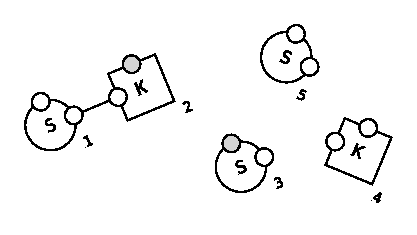
\includegraphics[scale=0.9]{figures/mixture.pdf}
  \end{center}
  \vskip -0.5cm
  \caption{An example of a reaction mixture. Instead of naming sites,
    we here identify them by their position on agents (phosphorylation
    sites are always shown on top). The relative position of agents in
    the figure is insignificant.  Phosphorylated sites are shown in
    gray.  Number labels correspond to global agent identifiers. }
  \label{fig:mixture}
\end{figure}


Interactions between agents are modeled by local rewriting
\emph{rules}.  A rule $r$ is defined by a triple
$(\RLHS{r}, \RRHS{r}, \lambda_r)$, where $\RLHS{r}$ is the left-hand
side specifying a pattern (the pre-condition), $\RRHS{r}$ the
right-hand side (or post-condition), and $\lambda_r$ a firing rate.
The basic idea is that the ``location" at which the mixture matches
$\RLHS{r}$ is rewritten in place by $\RRHS{r}$, changing the state of
the system. (Technically, a rule also requires a function from agents
in $\RLHS{r}$ to agents in $\RRHS{r}$ to make the rewrite
unambiguous.)

% -*- TeX-master: "ijcai18.tex" -*-

\begin{figure}[h]
  \vskip -0.2cm
  \begin{center}
    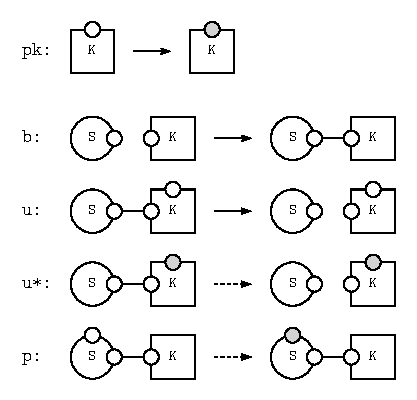
\includegraphics[scale=0.9]{figures/model.pdf}
  \end{center}
  \vskip -0.2cm
  % \caption{A motivating toy model. As usual in Kappa, sites not
  %   mentioned in a rule are left unchanged by it. Instead of naming
  %   sites, we here identify them by their position on an
  %   agent. Phosphorylated sites are shown in gray. Firing rates are
  %   not specified here but dotted arrows indicate \textit{slow}
  %   reactions, whereas solid arrows indicate \textit{fast} reactions.}
  \caption{A motivating toy model. Sites not mentioned in a rule are
    left unchanged by it. \longversion{As in
      Figure~\protect\ref{fig:mixture}, sites are identified by their
      position on an agent.}  Firing rates are not specified, but
    dotted (solid) arrows indicate \textit{slow} (\textit{fast})
    reactions
    $(\lambda_u \gg \lambda_{u^*} \approx \lambda_p)$.}
  \label{fig:model}
\end{figure}


In our toy model, agents are subject to the rules depicted in
Figure~\ref{fig:model}. Rule $b$ states that kinases and substrates
can bind, provided their requisite binding sites are free
(unbound). Note that $\RLHS{b}$ is a pattern: It omits mentioning the
sites that carry phosphorylation state, which are therefore not
considered when matching the mixture to $\RLHS{b}$. Rules $u$ and
$u^{*}$ define unbinding events that depend on the phosphorylation
state of the kinase $K$. The distinction is motivated by kinetics:
Rule $u$ fires at a much faster rate than $u^{*}$. Rule $p$ specifies
that a substrate can be phosphorylated when it is bound to a
kinase. For the sake of simplicity, we model the phosphorylation of a
kinase as a spontaneous process (rule $pk$).

By virtue of the $\lambda_r$, the rules of a model, together with an
initial mixture, constitute a dynamical system that we describe
shortly. We do so in a slightly nonstandard way by introducing the
auxiliary concept of an \emph{event template}. This is to prepare for
the insight in section~\ref{subsec:counterfactuals-semantics} that the
stochastic and deterministic aspects of a model's dynamics can be
cleanly separated, thus enabling counterfactual analysis.

An event template is a pair $(r, \xi)$ where $r$ is a rule and $\xi$ a
function from agents in $\RLHS{r}$ to global identifiers. We say that
$(r, \xi)$ is \emph{realizable} in mixture $m$ if the global
identifiers assigned by $\xi$ exist in $m$ and the agents bearing them
match $\RLHS{r}$. In this case, we write $\TRIGGERABLE{m}{(r, \xi)}$
(read ``$m$ admits $(r, \xi)$") and call $\xi$ an \emph{embedding} of
$\RLHS{r}$ into $m$:
\tryinline{\EMBS{r}{m} \eqdef \{ \xi \,:\,
  \TRIGGERABLE{m}{(r, \xi)}\}.}  Whenever $m \vdash (r, \xi)$, we
write $\UPDATE{m}{(r, \xi)}$ the mixture obtained by
realizing $(r, \xi)$, i.e.\@ by rewriting the agents with identifiers
in the codomain of $\xi$ into $\RRHS{r}$. The realization of an event
template at a particular time creates an (actual) \emph{event},
formally defined as a pair $(e, t)$ with $e$ an event template and $t$
its time of realization.

A model induces a continuous-time Markov chain (CTMC) over the
set of reachable mixtures, where state $m$ transitions to state
$\UPDATE{m}{(r, \xi)}$ at rate $\lambda_r$ for every event template
$(r, \xi)$ that is realizable in $m$. The rate of leaving state $m$ by
an application of rule $r$ is called the \emph{activity} $\alpha_r(m)$
of rule $r$ in
% \ifshort $m$: \else
mixture $m$ and is equal to the product of the rule's firing rate by
the number of embeddings of $\RLHS{r}$ into $m$:
% \fi
$\alpha_r(m)=\lambda_r|\EMBS{r}{m}|$. For example, in
Figure~\ref{fig:mixture}, rule $b$ has activity $2\lambda_b$ and rule
$u$ has activity $0$. The \emph{total activity} of a mixture is defined
as $\alpha(m)=\sum_r\alpha_r(m)=\sum_r\lambda_r|\EMBS{r}{m}|$.
% In terms of CTMC, it corresponds to the total transition rate of $m$.

The CTMC induced by a model can be simulated
with the \emph{Doob-Gillespie algorithm} \cite{gillespie1977exact},
which loops over the following steps:
\begin{inparaenum}[(1)]
\item draw a time interval $\delta$ to the next event from an
  exponential distribution with parameter $\alpha(m)$ and increment
  the simulated system time by $\delta$,
\item draw a rule $r$ with probability $\alpha_r(m)/\alpha(m)$ and
\item pick uniformly an embedding $\xi \in \EMBS{r}{m}$ of $L_r$ into
  $m$ and realize the event template $(r, \xi)$.
\end{inparaenum}
This algorithm is efficiently implemented for rule-based models in
Kappa as described in
\cite{DanosEtAl-APLAS07,BoutillierEK17}\longversion{; it is available
  at kappalanguage.org}. It outputs a sequence of events,
called a \emph{trace}.


\longversion{\begin{algorithm}
\caption{Doob-Gillespie algorithm}\label{alg:gillespie}
\begin{spacing}{1.2}
\begin{algorithmic}
\vspace{0.2cm}
  \STATE $t \gets 0$
  \STATE $m \gets\ $ initial mixture
  \vspace{0.1cm}
  \WHILE{ $t < t_\text{\,end}$ }
      \vspace{0.1cm}
      \STATE $\alpha \gets \sum_r {\lambda_r |\EMBS{r}{m}|}$
      \vspace{0.1cm}
      \STATE draw $\delta \sim \textsc{Exp}(\alpha) $
      \STATE $t \gets t + \delta$
      \STATE draw a rule $r$ with probability
      $\propto \ \lambda_r |\EMBS{r}{m}|$
      \STATE draw an embedding $\xi$ uniformly in $\EMBS{r}{m}$
      %\STATE update $m$ by triggering event $((r, \xi), t)$
      \STATE $m \gets \UPDATE{m}{(r, \xi)}$
      \STATE log event $((r, \xi), t)$
  \ENDWHILE
\vspace{0.1cm}
\end{algorithmic}
\end{spacing}
\end{algorithm}}

\subsection{Where Existing Analysis Falls Short}
\label{subsec:dumb-story}

% What about asking the question for the specific trace to make it
% clearer we are talking about actual causality ?

Consider our toy model and assume, for the sake of illustration, an
initial mixture $I$ with only a single kinase and a single substrate
whose sites are unbound and unphosphorylated. We then ask: Starting
from $I$, \emph{how} is $p$ typically achieved? We are not merely
looking for an account of reachability but for a causal explanation,
i.e.\@ a collection of events connected by causal influences.

For example, a simulation might produce the following trace (events
are labelled by the rules that induced them):
\begin{align}
  \label{example-trace} 
  b,\ \ u,\ \ pk,\ \ b,\ \ p,\ \ u^{*},\ \ \cdots
\end{align} 
Current techniques
\cite{DBLP:conf/fsttcs/DanosFFHH12,DanosEtAl-CONCUR07} generate a
causal account by first computing a \emph{sub-trace} of
(\ref{example-trace}) that is
\begin{inparaenum}[(i)]
\item \emph{valid} in the sense that each of its events can be
  triggered in turn starting from the initial mixture and
\item \emph{minimal} in the sense that none of its valid sub-traces
  features $p$.
\end{inparaenum}
The relations of enablement among events in the minimal sub-trace
yield a directed acyclic graph. Although trivial in our toy example,
minimization is an NP-hard problem. Carrying out this approach on
(\ref{example-trace}), one notes that the first occurence of $b$ sets
the necessary conditions for $p$, but these are subsequently undone by
$u$ only for the second occurrence of $b$ to re-introduce them. This
illustrates why minimization compresses a trace into events that are
\emph{necessary} for the outcome---which requires eliminating futile
cycles. In our case, the causal account for $p$ starts with the
initial condition, symbolized by the \emph{init} event, and skips to
the last $b$ before the $u$. Figure~\ref{fig:dumb-story} depicts the
resulting explanation graph, whose arrows denote enablement as defined
informally in section~\ref{sec:intro} and formally in
section~\ref{sec:inhibition}.

\begin{figure}[H]
  \vskip -0.8cm
  \begin{center}
    \includegraphics[scale=0.7]{figures/dot/dumb-story.pdf}
  \end{center}
  \vskip -1cm
  \caption{A causal explanation for $p$ in trace
    (\ref{example-trace}).  Events are labelled by the rules that
    induced them. The \emph{init} node corresponds to a special event
    that sets the mixture to its initial state.  }
  \label{fig:dumb-story}
\end{figure}


The problem is that the explanation depicted in
Figure~\ref{fig:dumb-story} fails to recognize the critical role of
$pk$ in the original trace. Given the rules of the model, one notes
that $p$ is slow and the average time that $K$ remains bound to $S$
depends on the phosphorylation state of $K$. The kinase $K$ is
phosphorylated in event $pk$, causing the complex between $K$ and $S$
to be sticky, giving the slow phosphorylation $p$ a chance to
occur. It seems reasonable to assert that $p$ would probably not have
happened had $pk$ not happened, since the opportunity for $p$ would
have been curtailed by a fast unbinding event. Thus, $pk$ should be
part of the explanation, although it neither enables $b$ nor $p$
directly (both rules are independent of $K$'s phosphorylation
state). Reasoning of this kind is \emph{counterfactual}
\cite{lewis1974causation,pearl2009causality}.

In section~\ref{sec:counterfactual}, we give a rigorous semantics to
this line of reasoning and introduce an algorithm for simulating
counterfactual scenarios. In section~\ref{sec:inhibition}, we show how
counterfactual dependencies between events can be systematically
explained in terms of a combination of enablement and prevention
arrows, leading to the explanation shown in Figure~\ref{fig:cex}. 
%for the counterfactual dependency between $p$ and $pk$ in our example.

%\section{Counterfactual simulation}

In this section, we derive a variation of the Gillespie algorithm for
simulating counterfactual traces. That is, given a reference trace
$\tau$ and an intervention $\iota$, we show how to simulate an
instance of $\CTRAJ{}$. Before we proceed, it is useful to refresh our
memory about the original Gillespie algorithm, which is summarized in
Listing~\ref{alg:gillespie}.


In Gillespie's algorithm, the activity of a rule $r$ is defined as the
product $\lambda_r|\EMBS{r}{M}|$ of its reaction rate by the number of
embeddings of its left hand side in the current reaction mixture.
Then, simulating a trace works by repeating the following steps:
\begin{inparaenum}[1)]
\item draw the time before the next simulation event from an
  exponential distribution of parameter the total activity $\alpha$ of
  the rules and increment the current time by this amount
\item draw a rule $r$ with probability proportional to its activity
\item pick an instance of the left hand side of $r$ uniformly in the
  current mixture and rewrite it.
\end{inparaenum}
A key property of Kappa's CTMC semantics that can be used to establish
the corectness of this algorithm is the following.
%
%
\begin{proposition}\label{prop:gillespie}
  Let $I=[t,\; t+\delta]$ a time interval and $m$ a mixture. Then,
  \[ \CProb{ T \cap I = \emptyset }{ \TSTATE{t}{T} = m } =
    e^{-\alpha(m) \cdot \delta} \] where $\alpha(m)$ is the total
  activity of mixture $m$.
\end{proposition}
%
%
% \input{proofs/gillespie-pty}
A similar theorem can be proved for counterfactual traces, involving a
modified notion of activity we call \emph{divergent activity}.
Indeed, suppose we are simulating a counterfactual trace and the
current mixture at time $t$ is $m$. Let $m_0$ the state of the
reference trace at time $t$. We say that a site is divergent if it has
different states in $m$ and $m_0$.  Besides, an embedding of the left
hand side of a rule $r$ into $m$ that features at least one divergent
site is said to be divergent. We write $\DEMBS{r}{m, m_0}$ the set of
all such embeddings.  Finally, we define the divergent activity of a
rule as the product of its rate by the number of divergent embeddings
of its left hand side into $m$ and write $\alpha'(m, m_0)$ the total
divergent activity:
\[\alpha'(m, m_0) = \sum_r \lambda_r |\DEMBS{r}{m, m_0}|. \]
Then, we can state the counterpart of Proposition~\ref{prop:gillespie}
for counterfactual simulation.
\begin{proposition}\label{prop:cosim-waiting}
  Let $\tau$ a trace and $\iota$ an intervention.  Let $I$ a time
  interval of width $\delta$ such that $\tau \cap I =
  \emptyset$. Then,
  \[
    \CProb{ \hat T_\iota \cap I = \emptyset } { T=\tau,\
      \TSTATE{t}{\hat T_\iota} = m\ } \,=\ e^{-\alpha'(m, m_0) \cdot
      \delta}
  \]
  where $m_0 = \TSTATE{t}{T}$ and $\alpha'(m, m_0)$ is the divergent
  activity of $m$ in respect to $m_0$.
\end{proposition}

% As summarized on Listing~\ref{alg:gillespie}, simulating a trace
% using Gillespie's algorithm works by repeating the following steps,
% starting from the initial mixture:

\begin{algorithm}
\caption{Doob-Gillespie algorithm}\label{alg:gillespie}
\begin{spacing}{1.2}
\begin{algorithmic}
\vspace{0.2cm}
  \STATE $t \gets 0$
  \STATE $m \gets\ $ initial mixture
  \vspace{0.1cm}
  \WHILE{ $t < t_\text{\,end}$ }
      \vspace{0.1cm}
      \STATE $\alpha \gets \sum_r {\lambda_r |\EMBS{r}{m}|}$
      \vspace{0.1cm}
      \STATE draw $\delta \sim \textsc{Exp}(\alpha) $
      \STATE $t \gets t + \delta$
      \STATE draw a rule $r$ with probability
      $\propto \ \lambda_r |\EMBS{r}{m}|$
      \STATE draw an embedding $\xi$ uniformly in $\EMBS{r}{m}$
      %\STATE update $m$ by triggering event $((r, \xi), t)$
      \STATE $m \gets \UPDATE{m}{(r, \xi)}$
      \STATE log event $((r, \xi), t)$
  \ENDWHILE
\vspace{0.1cm}
\end{algorithmic}
\end{spacing}
\end{algorithm} \newcommand{\EVF}[0]{e_{\text{f}}}
\newcommand{\EVCF}[0]{e_{\text{c}}}

\begin{algorithm}
\caption{Counterfactual resimulation}\label{alg:cosimulation}
\begin{spacing}{1.3}
\algsetup{indent=1.5em}
\begin{algorithmic}[1]
\vspace{0.2cm}
\STATE $t \gets 0$
\STATE $m \gets\ $ initial mixture
\WHILE{ $t < t_\text{\,end}$ }
  \STATE $m_0 \gets \TSTATE{t}{\tau}$
  \STATE $(\EVF{}, t_{\text{f}}) \gets $ first event of $\tau$ in time interval $(t, \infty)$
  \vspace{0.1cm}
  \STATE $\alpha' \gets \sum_r {\lambda_r |\DEMBS{r}{m, m_0}|}$
  \vspace{0.1cm}
  \STATE draw $\delta \sim \textsc{Exp}(\alpha') $
  \STATE $t_{\text{c}} \gets t + \delta$
  % \STATE
  \IF { $t_{\text{c}} < t_{\text{f}}$ }
      \STATE draw a rule $r$ with prob.
      $\propto \, \lambda_r |\DEMBS{r}{m, m_0}|$
      \STATE  draw a divergent embedding $\xi \in \DEMBS{r}{m, m_0}$
      \STATE {$e \gets (r, \xi)$}
      \IF {$ \neg \, \BLOCKED{\iota}{e, t_{\text{c}}} $ }
          \STATE $t \gets t_{\text{c}}$
          \STATE $m \gets \UPDATE{m}{e}$
          \STATE log event $(e, t)$
      \ENDIF
  \ELSE
      \STATE {$e \gets \EVF{}$}
      \STATE $t \gets t_{\text{f}}$
      \IF {$ \neg \, \BLOCKED{\iota}{e, t} $ \AND $ \TRIGGERABLE{m}{e} $ }
          \STATE $m \gets \UPDATE{m}{e}$
          \STATE log event $(e, t)$
      
      \ENDIF 
  \ENDIF
\ENDWHILE
\vspace{0.1cm}
\end{algorithmic}
\end{spacing}
\end{algorithm}


% \begin{theorem}[Corectness of resimulation]
%   Let $\tau$ a trace and $\iota$ an intervention.  We write
%   $R_\iota(\tau)$ the random variable defined by the resimulation
%   algorithm. Then, ${\hat T}_\iota \,|\, \{T = \tau\}$ and
%   $R_\iota(\tau)$ have the same probability law.
% \end{theorem}


\subsection{Deriving the cosimulation algorithm}

Suppose you are simulating a counterfactual trace for intervention
$\iota$ and reference trace $\tau$, that is, you are drawing an
instance of $\hat T_\iota \,|\, \{T=\tau\}$. Suppose you have already
simulated the first $t$ seconds of this counterfactual trace and you
want to know the time of the next event. Because both $T$,
$\hat T_\iota$ and $\Sigma$ are markovian, the only only relevant
information about what has already been simulated is the current state
of the counterfactual world $s := \TSTATE{t}{\hat T_\iota}$.


If we write $\delta$ the time difference between $t$ and the next
event after $t$ in $\tau$, we are interested in the following
probability:
\begin{equation}
  \CProb{ \hat T_\iota \cap [t, t+\delta) = \emptyset  }
  % { \underbrace{T=\tau, M = \mathcal{S}_t(\hat T_\iota)}_{\Delta} }
  { T=\tau,\, s = \TSTATE{t}{\hat T_\iota} }
\end{equation}
Writing $I = [t, t+\delta)$, this quantity can be rewritten as
follows:
\begin{align}
  \ & \ \CProb{ \hat T_\iota \cap I = \emptyset }
      { T=\tau,\, s = \TSTATE{t}{\hat T_\iota} } \\[0.5em]
  = & \ \CProb{ \bigwedge_{s \vdash e} (\,e \notin \Sigma \cap I \,)  }{ T=\tau } \\[1em]
  = & \ \prod_{s \vdash e}\, \CProb{e \notin \Sigma \cap I }{ T=\tau }
\end{align}
Indeed, given that $s = \TSTATE{t}{\hat T_\iota}$, no counterfactual
event happens in time interval $I$ if and only if no potential event
that is triggerable from state $s$ is scheduled in $I$.  Besides,
potential events are scheduled independently and so we can decompose
the resulting probability as a product.

Let $e$ a potential event such that $s \vdash e$. The probability that
$e$ has not been scheduled in $I$ given that $T=\tau$ depends on
whether or not $e$ is triggerable from state $s_0 :=
\TSTATE{t}{T}$. Indeed, we assumed that $\tau$ contains no event in
time interval $I$. Therefore, if $s_0 \vdash e$, then $e$ cannot be
scheduled in $I$, without which it would have been observed in $\tau$.
Thus,
\[ s_0 \vdash e \ \Rightarrow\ \CProb{e \notin \Sigma \cap I}{ T=\tau
  } = 1 \] Besides, if $s_0 \not\vdash e$, then the observation
$\{ T=\tau \}$ gives absolutely no information on whether or not $e$
has been scheduled in $I$ and so
\[ s_0 \not\vdash e \ \Rightarrow\ \CProb{e \notin \Sigma \cap I}{
    T=\tau } = e^{-\lambda_e \cdot \delta} \] as the scheduling
process of a potential event is a Poisson process. Combining these two
results with (4), we have:
\begin{align}
  \CProb{ \hat T_\iota \cap I = \emptyset }{ \Delta }
  =\ \prod_{s \vdash e, \, s_0 \not\vdash e} e^{-\lambda_e} = e^{-\alpha'(s, s_0)\cdot\delta}
\end{align}
where
\[\alpha'(s, s_0) := \sum_{s \vdash e, \, s_0 \not\vdash e}
  \lambda_e \] This quantity can be rewritten as follows:
\begin{align}
  \alpha'(s, s_0) &= 
                    \sum_{(r, \xi)} \textbf{1}\{ s \vdash (r, \xi),\ s_o \not\vdash (r, \xi) \}\cdot\lambda_r \\
                  &= \sum_r \lambda_r\sum_\xi \textbf{1}\{ s \vdash (r, \xi),\ s_o \not\vdash (r, \xi) \} \\
                  &= \sum_r \lambda_r |\DEMBS{r}{s, s_0}|
\end{align}
which gives us the definition of divergent activity. This result can
be summarized in the following theorem:
\begin{theorem} Let $\tau$ a trace and $\iota$ an intervention. Let
  $I$ a time interval of width $\delta$ such that
  $\tau \cap I = \emptyset$. Then,
  \[\CProb{ \hat T_\iota \cap I = \emptyset }{ T=\tau,\
      \TSTATE{t}{\hat T_\iota} = s\ }
    \ =\ e^{-\alpha'(s, s_0) \cdot \delta}
  \]
  where $s_0 = \mathcal{S}_t(\tau)$ and
  \[\alpha'(s, s_0) = \sum_r \lambda_r |\DEMBS{r}{s, s_0}| \]
  is the total divergent activity of $s$ with respect to $s_0$.
\end{theorem}
During normal simulation of a Kappa model, the activity of the
reaction mixture can be interpreted as its propensity to change. In
contrast, during counterfactual simulation, the divergent activity can
be interpreted as the propensity of the counterfactual mixture to
diverge from the reference mixture.






% $M_0 := \mathcal{S}_t(\hat \tau)$
% = \CProb{ \bigwedge_e (\,e \notin \hat T_\iota \cap [t, t+\delta)\,)  }{ \Delta } \\

%% -*- TeX-master: "ijcai18.tex" -*-

\section{Related Work}

We discussed at length in section~\ref{sec:counterfactual} how our
definition of counterfactuals in the context of rule-based models
relate to Pearl's standard account\cite{pearl2009causality}.

%\section*{Conclusions}

This paper proposes a methodology (and implementation) for giving meaning to counterfactual statements in the spirit of approaches based on structural equation models (SEMs) but in contexts where SEMs are not directly applicable. The case in point are rule-based models deployed with the goal of studying how a specific set of combinatorial and concurrent interactions underlie a complex process. Such problems are rampant in molecular systems biology. 

Structural equations represent explicitly (for example in terms of a
factor graph) aspects of the causal structure of a system. Yet, for
rule-based models that structure is implicit and has first to be
revealed. We argue that counterfactual statements play an important
role to this end. The challenge, then, is to give a semantics to
counterfactual statements when, unlike in SEM approaches, no explicit
causal structure is available to begin with. We break that impasse by
proposing a technique we call counterfactual simulation that is
cognate to the idea of counterfactual experiments in SEM. Using
counterfactual simulation, we show that causally explanatory diagrams
involving relations of enablement and prevention between events can be
constructed.

Our method leaves open many questions regarding best practices, which
we hope to address in future work. Such issues depend on the
availability of empirically meaningful models. On a more conceptual
side, we wonder whether explanatory diagrams, such as
Figure~\ref{fig:cex}, constructed via counterfactual experiments as we
define them here might constitute a basis for obtaining structural
equations from complex models. These equations would always be
relative to an outcome of interest defined at the outset. Replacing a
rule-based model with such equations could enable targeted statistical
analysis to estimate model parameters, for which simulations would be
too expensive.

%\section*{Acknowledgments}

\ifshort This work was sponsored by the Defense Advanced Research
Projects Agency (DARPA) and the U. S. Army Research Office under grant
numbers W911NF-14-1-0367 and W911NF-17-1-0073.  We are grateful to
Pierre Boutillier for his help in implementing counterfactual
resimulation. We thank J\'{e}r\^{o}me Feret, Matt Fredrikson,
Micka\"{e}l Laurent and Jean Krivine for valuable discussions and
insights. We thank Thomas Kolokotrones, Ariel Procaccia and the
anonymous reviewers for precious feedback.

\else

This work was sponsored by the Defense Advanced Research Projects
Agency (DARPA) and the U. S. Army Research Office under grant numbers
W911NF-14-1-0367.  The views, opinions, and/or findings
contained in this report are those of the authors and should not be
interpreted as representing the official views or policies, either
expressed or implied, of the Defense Advanced Research Projects Agency
or the Department of Defense. 

We are grateful to Pierre Boutillier, the maintainer of the Kappa
simulator, for his help in implementing counterfactual resimulation.
We thank J\'{e}r\^{o}me Feret, Jean Krivine, Matt Fredrikson and
Micka\"{e}l Laurent for valuable discussions and insights.  Finally,
we thank J\'{e}r\^{o}me Feret, Thomas Kolokotrones and Ariel Procaccia
for valuable feedback on our draft.
\fi


%%%%%%%%%%%%%%%%%%%%%%%%%%%%%%%%%%%%%%%%%%%%%%%%%%%%%%%%%%%%%%%%%%%%%%%%%%%%%%%%

% \appendix

%% The file named.bst is a bibliography style file for BibTeX 0.99c
\nocite{*}
\bibliographystyle{named}
\bibliography{ijcai18}

\end{document}

%%%%%%%%%%%%%%%%%%%%%%%%%%%%%%%%%%%%%%%%%%%%%%%%%%%%%%%%%%%%%%%%%%%%%%%%%%%%%%%%
